\chapter{Testes}

Nesse capítulo veremos como o teste está diretamente ligado à qualidade de software, os principais tipos de testes, conceitos e ferramentas de automação, veremos quais os tipos de testes que serão aplicados ao nosso projeto e a importância da infra-estrutura de testes em um projeto.


\section{Definição}

Segundo o dicionário de termos da IEEE, teste é definido da seguinte forma:

\begin{itemize}
	\item Teste: atividades nas quais um sistema ou um componente é executado sob determinadas condições e os resultados são observados ou gravados, e uma avaliação é feita observando determinado comportamento do sistema ou do componente;
\end{itemize}

\section{Teste de Software e Qualidade de Software}

O teste de software está diretamente ligado com a qualidade do software que está sendo desenvolvido. Podemos ver essa ligação já na definição de qualidade de software.

\begin{itemize}
	\item Qualidade de Software: Conformidade a requisitos funcionais e de desenvolvimento explicitamente declarados, a padrões de desenvolvimento claramente documentados e a características implícitas que são esperadas de todo software profissionalmente desenvolvido.
\end {itemize}

Dentro da qualidade de software temos a atividade de garantia de qualidade de software e esta compreende uma variedade de tarefas associadas a sete grandes atividades, entre elas a atividade de testes:

\begin{enumerate}
	\item Aplicação de métodos técnicos;
	\item realização de revisões técnicas formais;
	\item Atividades de testes de software;
	\item Aplicação de padrões;
	\item Controle de mudanças;
	\item Medição;
	\item Manutenção de registros e reportagem;
\end{enumerate}

Então podemos estar certos de que se queremos um software que atenda aos requisitos especificados, funcionais e não funcionais, que possua uma quantidade de erros reduzida e um desempenho que atenda ao usuário, uma tarefa que não pode ser despensada é o teste da aplicação. Como já dito anteriormente, teste de software e qualidade de software estão intimamente ligados, na tabela ~\ref{tab:testequalidade} podemos ver quais as características de qualidade são verificadas por determinados tipos de testes.

\begin{table}
	\caption{Tipos de teste e sua característica de qualidade correspondente}
	\begin{center}
	\begin{tabular}{ccc}
		\hline
			\textbf{Tipos de Teste} & \textbf{Características de qualidade} \\
		\hline
			Funcionalidade & Funcionalidade \\
			Interfaces & Conectividade \\
			Carga & Continuidade, Performance \\
			Produção & Operabilidade \\
			Recuperação & Recuperação \\
			Regressão id & Todas \\
			Segurança & Segurança \\
		\hline
	\end {tabular}
	\end{center}
	%\caption{Fonte: http://docs.mongodb.org}
	\label{tab:testequalidade}
\end{table}

\section{Tipos de Testes}


%Segundo Ian Sommerville, o teste de componentes e o teste de sistema são as duas atividades fundamentais do teste de %software. Enquanto o teste de componentes testa as partes da aplicação, o teste de sistema testa a aplicação como um todo.

O teste de software nos permite trabalhar com diversas estratégias e em diferentes níveis da aplicação. Emerson Rios e Trayahú Moreira ~\cite{rios2006teste} dizem que muitas vezes os tipos de software se sobrepõem, sendo até mesmo as suas definições abrangentes ou específicas, confome sua execução. Nessa seção listaremos os principais tipos de testes descritos por esses autores.

\subsection{Aplicados a cada estágio de teste}

\subsubsection{Testes Caixa Preta}

Esse tipo de teste tem como objetivo verificar as funcionalidades da aplicação e a aderência aos requisitos, do ponto de vista do usuário, sem se basear no código ou lógica interna da aplicação.

\subsubsection{Testes Caixa Branca}

Os testes de caixa branca avaliam o código, a lógica interna do componente, as configurações e outros elementos técnicos.

\subsection{Estágios (ou Níveis) de teste}

\subsubsection{Testes unitários}

Esse é o tipo de teste que analisa o estágio mais baixo da aplicação. São aplicados nos menores componentes de código criados, verificando o atendimento as especificações e funcionalidades. Verificam o funcionamento de um pedaço do sistema, componente ou programa,  isoladamente. Geralmente são realizados pelos próprios desenvolvedores.

\subsubsection{Testes de integração}

Esse teste visa testar se as interações estre os componentes da aplicação está resultando em algum tipo de erro. Tem como objetivo assegurar que as interfaces funcionem corretamente e que os dados são processados corretamente.Componentes podem ser pedaços de código, módulos, aplicações distintas, clientes e servidores etc. Esse tipo de teste possui várias estratégias. Podemos testar a integração desde os componentes de mais baixo nível (Booton-up)  até o sistema como um todo (Teste de sistema). Para o nosso trabalho nos atentaremos ao teste de sistema.

\subsubsection{Testes de sistema}

Esse teste é executado sobre o sistema como um todo, ou um subsistema, dentro de um ambiente operacional controlado. Deve ser simulada a operação normal do sistema, sendo testadas todas as suas funções de forma mais próxima possível do que irá ocorrer no ambiente de produção. É nesse estágio que deve-se realizar os testes de carga, performance, usabilidade, compatibilidade, segurança e recuperação.

\subsubsection{Testes de aceitação}

São realizados pelos usuários e visam garantir que a solução atenda aos objetivos do negócio e a seus requisitos, verificando as funcionalidades e a usabilidade do software.

\subsection{Outros tipos de testes}

%\subsubsection{Testes de regressão}

\subsubsection{Testes Back-to-back}

É quando o mesmo teste é executado em versões diferentes do software e os resultados são comparados.

\subsubsection{Testes de Configuração}

É nesse tipo de teste de a execução da aplicação é analisada em diferentes configurações de ambiente.

\subsubsection{Testes de Usabilidade}

Mede a facilidade de uso da aplicação pelos usuários. É mais comum em aplicações web.

\subsubsection{Testes de Segurança}

Verifica o quão segura é a aplicação a acesso de usuários não autorizados.

\subsubsection{Testes de Recuperação}

Mede a qualidade da recuperação do software após falhas de hardware ou outro problemas inesperados.

\subsubsection{Testes de Compatibilidade}

Verifica se um software é capaz de ser executado em um ambiente determinado.

\subsubsection{Testes de Desempenho}

Verifica a adequação da aplicação aos níveis de desenpenho e tempo de resposta definidos nos requisitos. Também são conhecidos como testes de performance.

%\subsubsection{Testes Alfa e Beta}



\section{Testes de Carga e de Performance}

Como o objetivo do trabalho é medir o desempenho da nossa aplicação com o uso de diferentes bancos de dados, restringimos os testes que serão usados no nosso projeto aos testes de carga e performance.

\subsection{Testes de carga}

Permite avaliar a aplicação sob uma alta carga de dados, repetidas entradas de dados, consultas complexas ou uma grande quantidade simultânea de usuários. Dessa forma é possível medir o nível de escalabilidade da aplicação. Esse tipo de teste deve ser aplicado durante os testes de sistema e também podem ser chamados de testes de estresse.


\subsection{Teste de Performance}

Molyneaux fala que do ponto de vista dos usuários, uma aplicação possui boa performance quando ela o permite realizar determinada tarefa sem demora~\cite{theartoftestperf}. Ela ainda diz que em uma aplicação performática o usuário nunca poderá se deparar com uma tela vazia ao realizar operações. O teste de performance é usado para medir o desempenho, em tempo de execução, e com todos os módulos integrados. Conforme Molyneaux, dividiremos os requisitos de performance em dois: orientados a serviço e orientados a eficiência.%citar o livro de engenharia de software pressman

Os indicadores de performance orientados a serviço são a disponibilidade e o tempo de resposta. Eles medem a qualidade do serviço que a aplicação está provendo ao usuário. Já os indicadores orientados a eficiência são a vazão e utilização. Vamos definir esses termos:

\begin{itemize}
\item Disponibilidade: É a característica de estar disponível para o usuário. Em softwares críticos, qualquer período de indisponibilidade pode gerar grandes prejuísos.
\item Tempo de resposta: É o intervalo de tempo entre a requisição e a resposta da aplicação. 
\item Vazão: É a taxa em que os eventos da aplicação ocorrem.
\item Utilização: É a porcentagem da capacidade total de recursos da aplicação que esta sendo usada.
\end{itemize}

Para que o nosso processo de teste de performance seja bem sucedido precisamos seguir algumas etapas.

\begin{enumerate}
\item Escolher uma ferramenta de teste de performance apropriada;
\item Desenvolver um ambiente de teste adequado a realidade dos testes e o mais próximo da realidade;
\item Escolher os objetivos que desejamos alcançar no trabalho;
\item Identificar e criar scripts para as transações críticas para o negócio;
\end{enumerate}


\section{Automação de Testes}

Durante muito tempo os testes de software foram feitos manualmente. Os proprios programadores eram encarregados de simular as mais diversas situações ~\cite{rios2006teste}. Com o passar do tempo as aplicações se tornaram muito mais complexas e, consequentemente, o processo de teste manual se tornou inviável. Esse cenário foi ideal para que surgissem ferramentas de automação do processo de testes.

	\begin{figure}[!htbp]
		\begin{center}
			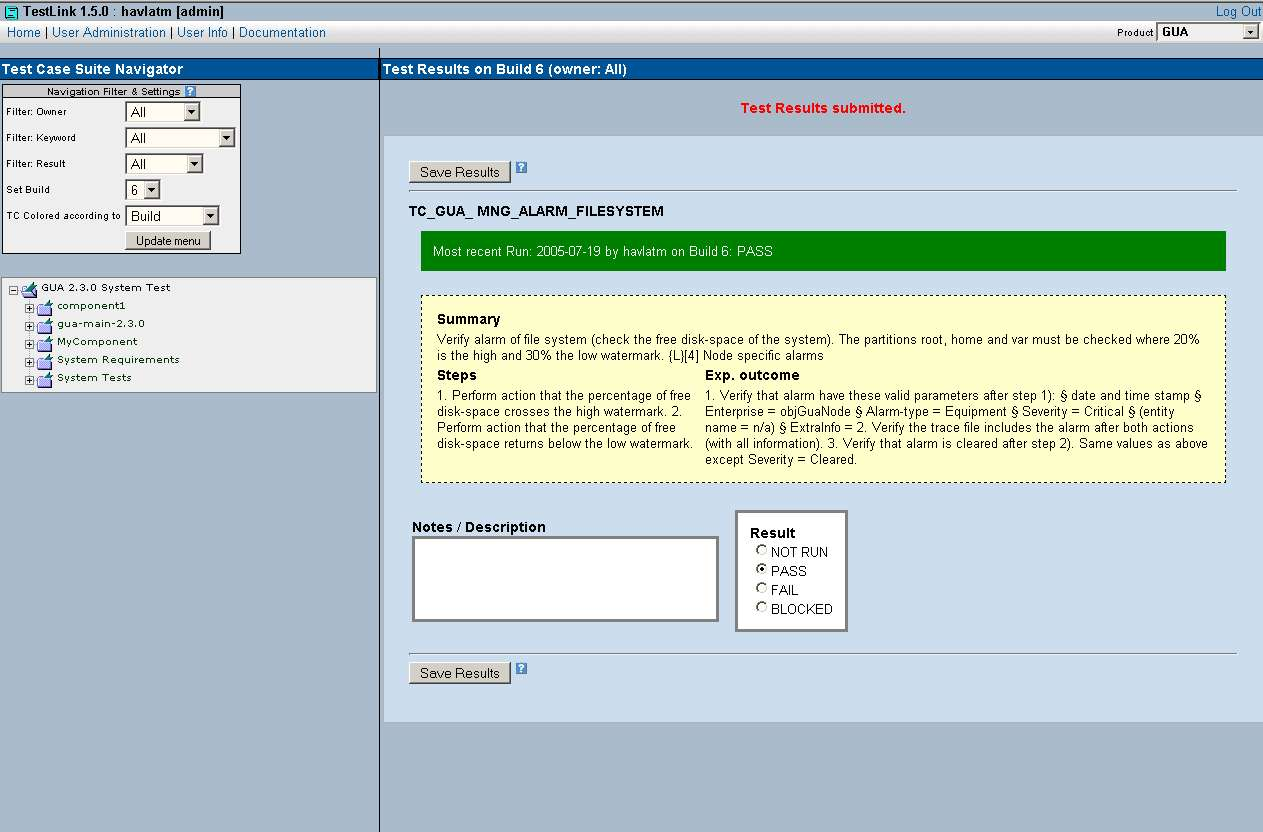
\includegraphics[width=0.8\textwidth]{testlink}
		\end{center}
		\caption{TestLink - acompanhamento/suporte ~\cite{siteTestLink}}
		\label{fig:testlink}
	\end{figure}

As ferramentas de automação de teste visam facilitar o processo de teste e podem auxiliar no desenvolvimento dos testes, execução, manuseio das informações de resultado e a comunicação entre os envolvidos no processo. Utilizando scripts essas ferramentas são capazes de simular a utilização da aplicação por um ou vários usuários e, além disso, podem ser simulados vários cenários de uso. As ferramentas de teste podem ser divididas em três grupos: desenvolvimento, execução ~\ref{fig:jmeter} e acompanhamento/suporte ~\ref{fig:testlink}.

	\begin{figure}[!htbp]
		\begin{center}
			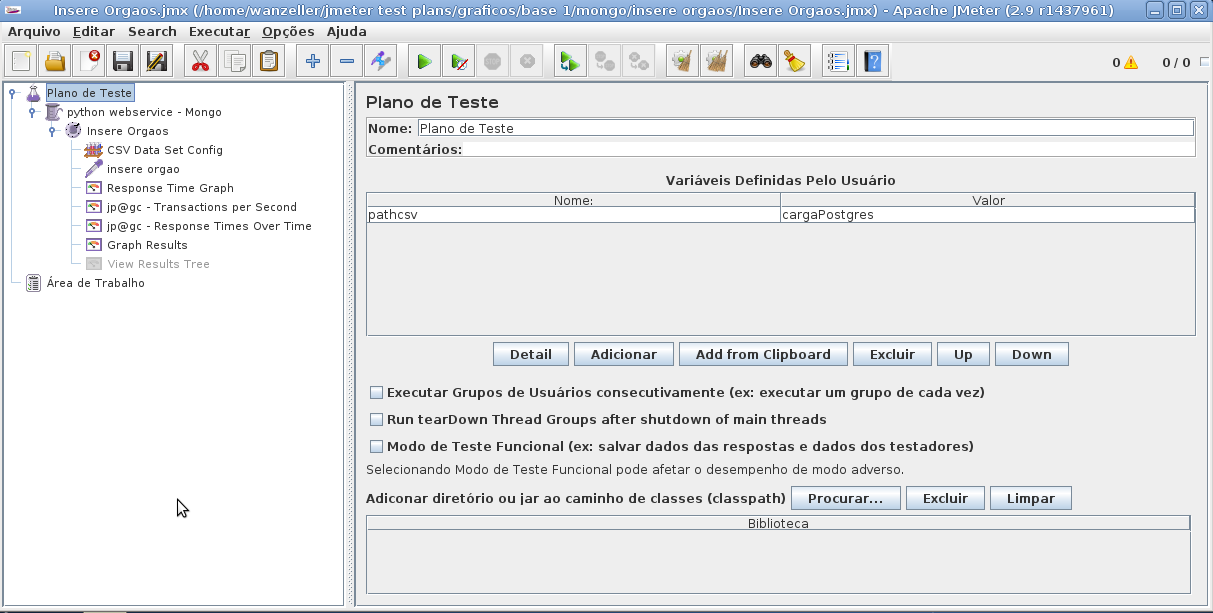
\includegraphics[width=0.8\textwidth]{jmeter}
		\end{center}
		\caption{JMeter - Ferramenta para execução de testes ~\cite{siteJmeter}}
		\label{fig:jmeter}
	\end{figure}


\section{JMeter}

O Apache JMeter é uma aplicação open source, 100\% desenvolvida em java e que foi criada para a execução de testes de carca e para medição de performance. Foi originalmente criado para testar aplicações web. O JMete pode ser usado para testar a performance tanto de recursos estáticos quanto de recursos dinâmicos  (arquivos, servelts, scripts Perl, objetos Java, Bancos de dados e queries, Servidores FTP e etc ). Com ele é possível simular cargas pesadas em um servidor, rede ou objeto para testar o seu comportamento ou para analisar a performance em diferentes tipos de carga ~\cite{siteJmeter}.

O JMeter pode testar diferentes tipos de servidores como:

\begin{itemize}
\item Web - HTTP, HTTPS
\item SOAP
\item Database via JDBC
\item LDAP
\item JMS
\item Mail - SMTP, POP3 e IMAP
\item Comandos nativos ou scripts shell
\end{itemize}

Para realizarmos testes no JMeter precisamos criar um plano de teste. O plano de teste descreve uma série de passos que o JMeter terá de executar. O plano de teste pode conter os seguintes elementos: Grupo de Thread, controladores lógicos, testadores, ouvintes, timers, assertions e elementos de configuração. A seguir vamos ver os elementos que serão usados nos planos de teste desse trabalho.

\subsection{Testador}

Quando iniciamos o nosso plano de teste, o primeiro item que devemos procurar é o testador. Os testadores basicamente enviam requisições aos servidores e aguardam retorno. Cada testador possui diversas configurações que podem ser customizadas.

\subsubsection{Requisição SOAP/XML - RPC}

O testador SOAP (figura \ref{fig:testador_insere_orgao}) é usado para mandar requisições SOAP para um Web service.  Ele cria uma requsição HTTP POST com os dados especificados e executa o POST.  As principais configurações são:


\begin{itemize}
\item \textbf{URL}:  Endereço do WSDL do Web service.
\item \textbf{Ação SOAP}: Endereço da requisição SOAP que o testador utilizará.
\item \textbf{Dados SOAP/XML-RPC}: Requisição que será enviada para o Web service. Deve estar em formato XML.
\end{itemize}

	\begin{figure}[!htbp]
		\begin{center}
			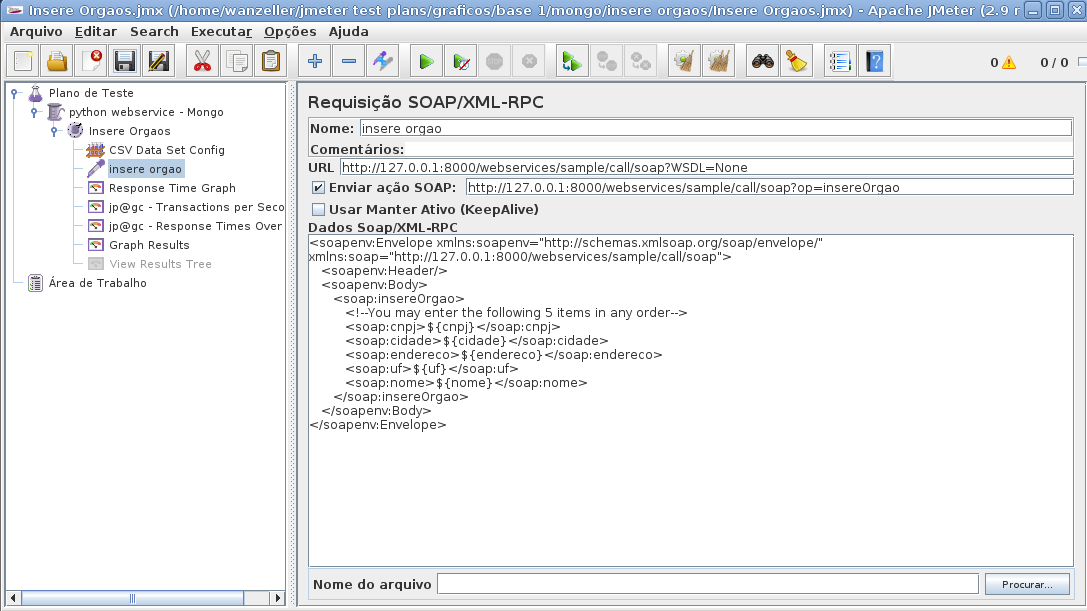
\includegraphics[width=1\textwidth]{testador_insere_orgao}
		\end{center}
		\caption{Testador de Requisição SOAP/XML - RPC}
		\label{fig:testador_insere_orgao}
	\end{figure}

\subsection{Ouvintes}

Os ouvintes nos permite ter acesso às informações geradas pelo JMeter durante os testes. Temos ouvintes que geram gráficos, gravam informações em arquivos, listam as responses e outros vários.

\subsubsection{Gráfico de Resultados}

O gráfico de resultados gera um gráfico com os tempos de todas as requisições. Na legenda do gráfico temos o tempo da requisição atual (preto), a média atual de todas as requisições (azul), a derivação atual (vermelho), e a vazão atual (verde), todas em milisecundos. A vazão representa o número de transações por minuto (os atrazos causados pelo processamento interno do JMeter não são considerados).

\subsubsection{Gráfico de Tempo de Resposta}

O gráfico de tempo de resposta plota uma linha no gráfico que descreve a evolução do tempo de resposta de cada requisição durante o teste.

\subsection{Elemento de Configuração}

Os elementos de configuração podem ser utilizadoos para configurar padrões e variáveis que serão utilizadas pelos testadores.

\subsubsection{Configuração de Dados CSV}

Esse elemento de configuração é usado para ler linhas de um arquivo e armazená-las em variáveis.Podemos ver um exemplo na figura \ref{fig:configuracao_csv}. Para realizar os testes de inserção de dados no banco esse elemento será de grande importância.

	\begin{figure}[!htbp]
		\begin{center}
			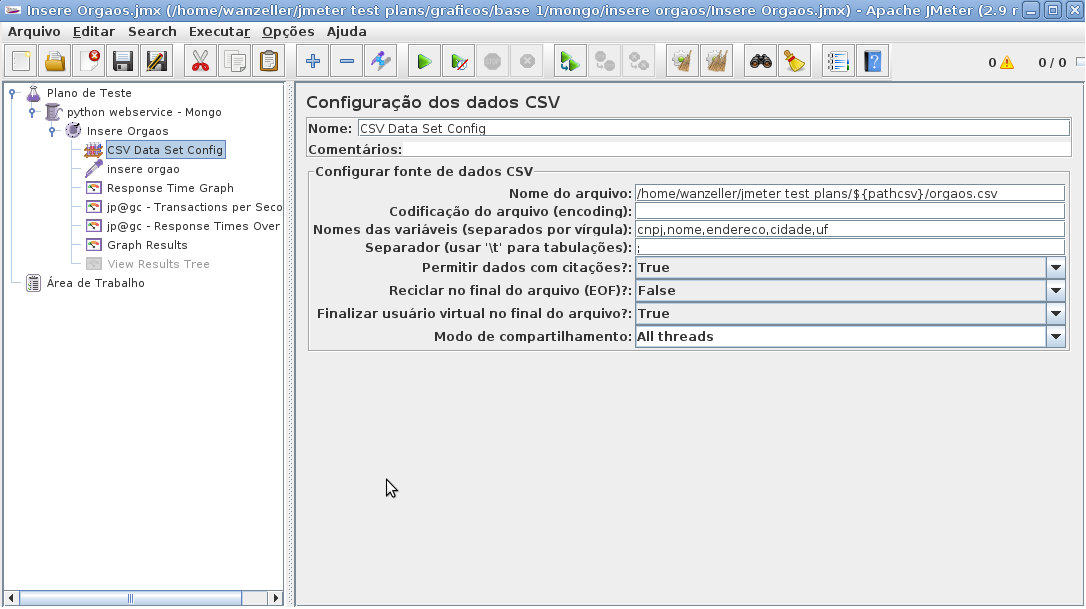
\includegraphics[width=1\textwidth]{configuracao_csv}
		\end{center}
		\caption{Elemento de Configuração de Dados CSV}
		\label{fig:configuracao_csv}
	\end{figure}

%\section{Infra-estrutura de Testes}














